\section{Results}
\label{sec:results}

Unless stated otherwise, results use the QFF synthetic noise model and are averaged over five random payloads; error bars are standard deviations over payloads. Numbers quoted for ``the game'' refer to the single payload (seed 7) that the game uses.

\subsection{Validation}
\label{sec:res-val}
Figure~\ref{fig:validation} compares the exact evaluation with 50{,}000-shot \texttt{SamplerV2} runs for twenty configurations. The kept fractions agree within \ValKeepSigma{} standard errors in the worst case, and the classical fidelities of the post-selected distributions agree to within \ValHdiff. Noiseless runs confirm that every check found by \texttt{qiskit-paulice}, and every check after safe-zone doping, has a false-alarm rate that is numerically zero (below $10^{-9}$ in all \NumMoves{} moves), while each check broken by blind doping fires on perfect runs with probability between 0.15 and 0.69 (median 0.25). For Clifford payloads the stabilizer-group identity and the statevector overlap give the same $F_0$ to within \ValStabDiff.

\begin{figure}[t]
\centering
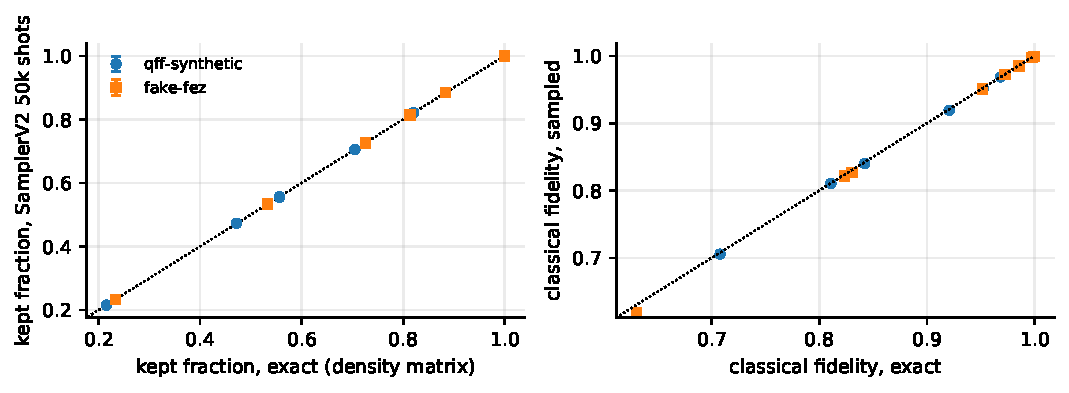
\includegraphics[width=\columnwidth]{figures/fig_validation}
\caption{Exact density-matrix numbers against 50{,}000-shot runs of the Aer \texttt{SamplerV2} primitive, for twenty configurations and both noise models. Error bars are two standard errors.}
\label{fig:validation}
\end{figure}

\subsection{How many checks? A break-even depth}
\label{sec:res-k}
Figure~\ref{fig:checks} follows one call of \texttt{add\_pauli\_checks} that commits checks on qubits 0 to 5 one at a time. More checks always raise the post-selected fidelity and always lower the kept fraction, as expected. The interesting quantity is the gain in fidelity rate, $G=R_{1/2}/F_0$. At depth 18 the fidelity rises from \EoneFzeroDeep{} without checks to \EoneFpsDeep{} with the best number of checks ($k=\EoneKDeep$) while \EoneKeepDeep{} of the shots survive, a gain of \EoneGainDeep. At depth 12 the best gain is \EoneGainMedium{} ($k=\EoneKMedium$). At depth 6 no number of checks beats the unprotected circuit in this sweep: one check already gives $G=\EoneGainOneShallow$, and every further check lowers the rate. Choosing the targets carefully helps only a little; the best move in the game's shallow Clifford level, checks on \BestShallowTZeroTargets, gains a factor of \BestShallowTZeroGain{} (Table~\ref{tab:best}).

The reason is a budget argument. A check adds two to five CZ gates, each of which can fail with probability $p_2$, and it can only catch errors that occur on the wires its flow monitors. On a shallow circuit there are few errors to catch, so the check's own gates are a large fraction of the total noise, and most of what the extra checks catch are errors that the checks themselves introduced. As the circuit gets deeper the payload contributes more and more of the noise, and the same ancilla becomes a better investment. The game makes this visible: in the shallow levels the best possible score is barely above the score of posting no sentinel at all, and most moves score below it.

\begin{figure*}[t]
\centering
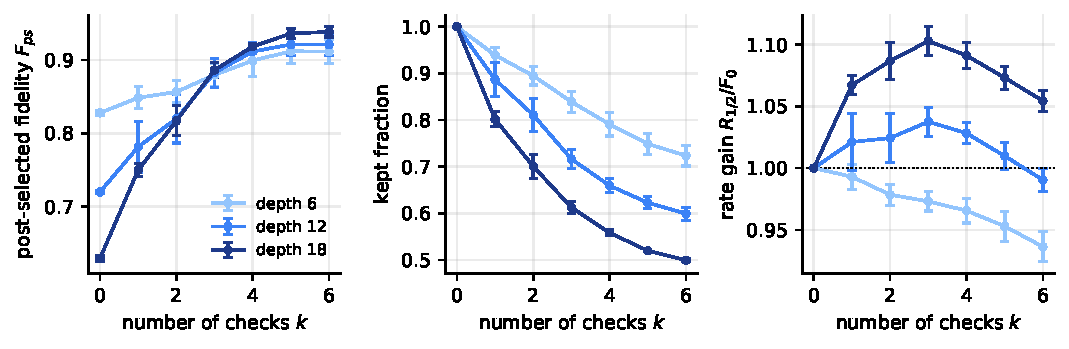
\includegraphics[width=0.9\textwidth]{figures/fig_check_count}
\caption{Post-selected fidelity, kept fraction and fidelity-rate gain $R_{1/2}/F_0$ against the number of checks committed by \texttt{add\_pauli\_checks} (targets 0 to 5 in order), for three depths. Five payloads; error bars are standard deviations. The dotted line marks break-even.}
\label{fig:checks}
\end{figure*}

\subsection{$T$ count against check placement}
\label{sec:res-t}
Figure~\ref{fig:tcount} is the central result. A fixed set of three checks (on qubits 0, 2 and 4) protects payloads doped with up to 16 $T$ gates, placed with each of the three policies. Without checks, the $T$ gates barely change the fidelity: at depth 18 $F_0$ moves from \EtwoNoneFzeroTZeroDeep{} with no $T$ gate to \EtwoNoneFzeroTSixteenDeep{} with sixteen, because the $T$ gates themselves are noiseless and only slightly change how the existing errors propagate. With safe-zone doping, the post-selected fidelity and the kept fraction are flat as well: the checks see exactly the same faults whether or not the $T$ gates are present, which is the invariance exploited in Ref.~\cite{martiel2026sampling}. The largest drop in $F_{\mathrm{ps}}$ between the Clifford circuit and its 16-$T$ safe-zone version is \EtwoSafeDrift{}, the footprint of errors that were harmless before doping and are harmful after it.

Blind doping tells a different story. Each $T$ that lands on a wire where some check flow acts as $X$ or $Y$ breaks that check. With only four $T$ gates at depth 18, blind placement breaks on average \EtwoBrokenFourDeep{} of the three checks. A broken check fires on perfect runs, so post-selecting on it throws away good shots: at depth 18 with 16 $T$ gates, the kept fraction falls to \EtwoBlindKDeepTSixteen{} and the post-selected fidelity to \EtwoBlindFDeepTSixteen, against \EtwoSafeKDeepTSixteen{} and \EtwoSafeFDeepTSixteen{} with safe-zone doping. Post-selecting on a broken check is a projection onto one eigenspace of an operator that no longer stabilizes the ideal state, and that projection rotates the state away from the target.

The third policy is the one most players reach for: if a check is broken, stop listening to it. This is worse still. With 16 $T$ gates at depth 18 the fidelity of blind doping with retirement is \EtwoRetireFDeepTSixteen, below the \EtwoNoneFDeepTSixteen{} of the circuit with no checks at all. The ancilla of a retired check is still entangled with the data through a flow that no longer closes, so discarding its outcome amounts to measuring a non-stabilizer Pauli operator and forgetting the result. That is a dephasing channel on the data, and it destroys exactly the coherence that the $T$ gates were meant to create. A broken check cannot be switched off after the fact; it has to be removed from the circuit or never broken in the first place.

\begin{figure*}[t]
\centering
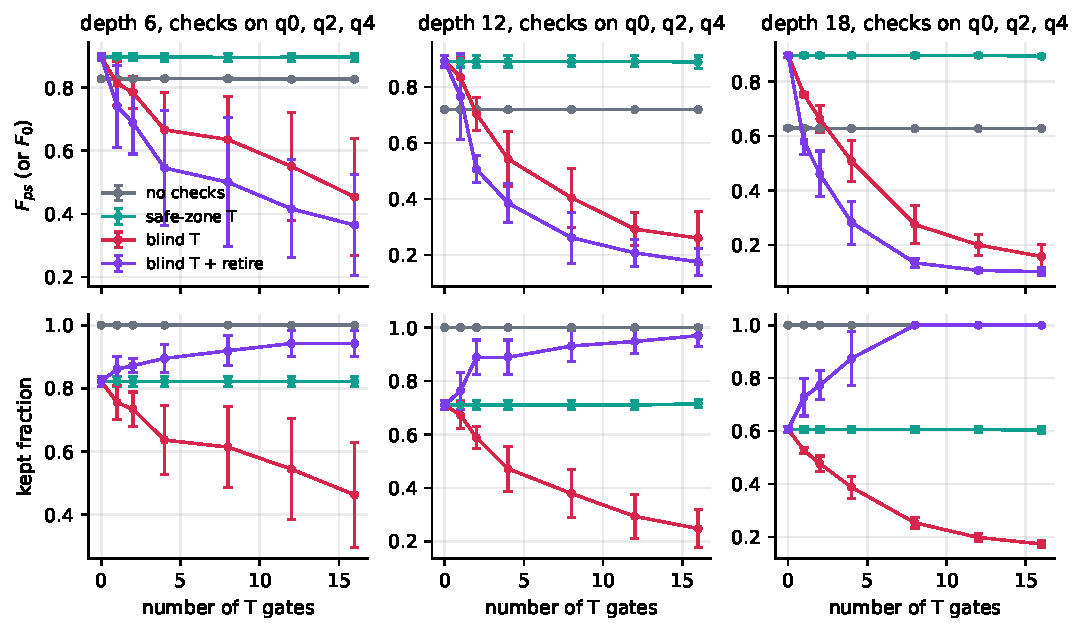
\includegraphics[width=0.95\textwidth]{figures/fig_t_count}
\caption{$T$ count against check placement. Top: post-selected fidelity (or $F_0$ without checks); bottom: kept fraction; columns: depth 6, 12, 18. Checks on qubits 0, 2, 4. Safe-zone doping (teal) is flat; blind doping (red) breaks checks; retiring broken checks (purple) is worse than having no checks (grey).}
\label{fig:tcount}
\end{figure*}

\subsection{Magic capacity: protection and magic compete}
\label{sec:res-cap}
If safe-zone doping is free, why not always use it? Because the safe zones shrink as checks are added. Figure~\ref{fig:capacity} counts the Z-safe sites for every one of the 64 target sets at four depths. At depth 18 all \CapTotalDeep{} sites are safe without checks; with two checks \CapDeepTwo{} remain on average, with four \CapDeepFour{}, and with six only \CapDeepSix. A check is useful precisely because its flow acts as $X$ or $Y$ on many wires, where it catches $Z$ errors, and those are exactly the wires where a $T$ gate would break it. Protection against phase errors and room for magic are two uses of the same spacetime, and one can only be bought at the expense of the other.

In the game this shows up as illegal moves. Across all levels \NumIllegal{} moves are illegal because there are fewer safe sites than $T$ gates to place, all of them in the levels with 16 $T$ gates. The optimum moves accordingly. In the game's deep level, the best move with up to eight $T$ gates uses three checks (\BestDeepTEightTargets), while with sixteen $T$ gates the best move drops to \BestDeepTSixteenTargets: one fewer check, to free enough safe sites for the magic. The gain falls from \BestDeepTEightGain{} to \BestDeepTSixteenGain. This is the non-obvious trade-off asked for by the challenge in its plainest form: the right number of checks depends on how much magic the circuit carries.

\begin{figure*}[t]
\centering
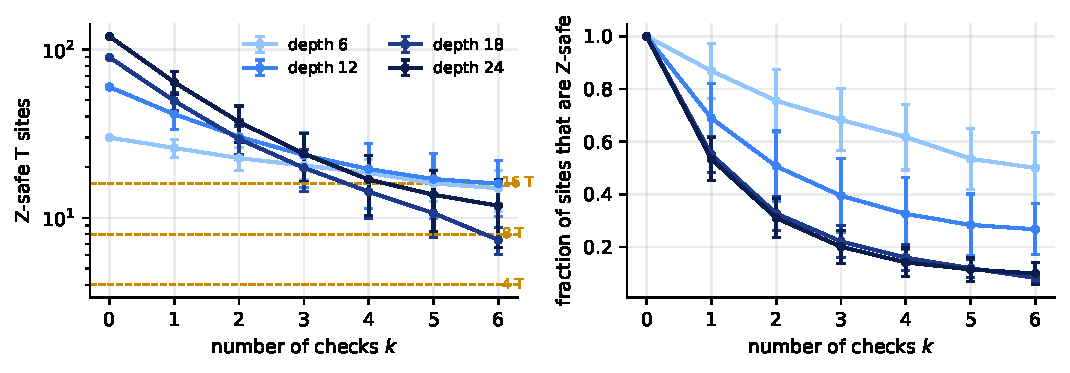
\includegraphics[width=0.9\textwidth]{figures/fig_capacity}
\caption{Magic capacity. Left: number of Z-safe $T$ sites against the number of checks, averaged over all target sets of that size and five payloads (log scale; dashed lines mark $T$ demands of 4, 8 and 16). Right: the same as a fraction of all sites.}
\label{fig:capacity}
\end{figure*}

\subsection{The best trade-off, and why it wins}
\label{sec:res-best}
Table~\ref{tab:best} lists the best move of every level of the game under the default shot price $\beta=1/2$. Three features stand out. First, the winning moves never use blind doping when the quota is four or more: as soon as a check can be broken, protecting it pays more than any extra coverage. Second, the winning moves use two or three checks, never four. The fourth check adds gates for little extra coverage, the same diminishing return seen in the $\gamma$ cost and in Fig.~\ref{fig:checks}. Third, which qubits are guarded matters almost as much as how many. With two checks on the deep payload the gain ranges from \LocMinDeep{} to \LocMaxDeep{} depending on the targets (Fig.~\ref{fig:location}). The $\gamma$ cost used by \texttt{qiskit-paulice} ranks checks for a fixed target, but it does not choose the targets; the player does, and a poor choice of targets can waste most of the benefit.

Why does the deep, four-$T$ winner (\BestDeepTFourTargets, safe zones) win? It raises the fidelity from \BestDeepTFourFzero{} to \BestDeepTFourFps{} while keeping \BestDeepTFourKeep{} of the shots. Its three checks sit on qubits whose flows overlap little, so together they cover a large share of the two-qubit faults, and the rejection rate is close to the probability that a fault occurred at all. Adding a fourth check would catch fewer new faults than its own gates create, and any extra check would also remove safe sites. The move sits on the Pareto front of the level (Fig.~\ref{fig:pareto}), at the point where the curve of constant $R_{1/2}$ touches it.

The shot price changes the answer (Fig.~\ref{fig:pareto}, right). At $\beta=0$, where only purity counts, the best move uses all four checks at every depth; at $\beta=1$, where every discarded shot counts fully, it uses none. The default $\beta=1/2$ is the only one of the three with an operational meaning (Sec.~\ref{sec:score}), and it is the one in which spacetime detection is worth something on deep circuits and nothing on shallow ones.

\begin{table}[t]
\caption{Best move of each level of the game (payload seed 7, QFF synthetic noise, $\beta=1/2$). $G=R_{1/2}/F_0$.}
\label{tab:best}
\begin{ruledtabular}
\begin{tabular}{cclccc}
$d$ & $n_T$ & checks, placement & $F_0$ & $F_{\mathrm{ps}}$ ($\kappa$) & $G$ \\
\hline
\BestTableRows
\end{tabular}
\end{ruledtabular}
\end{table}

\begin{figure*}[t]
\centering
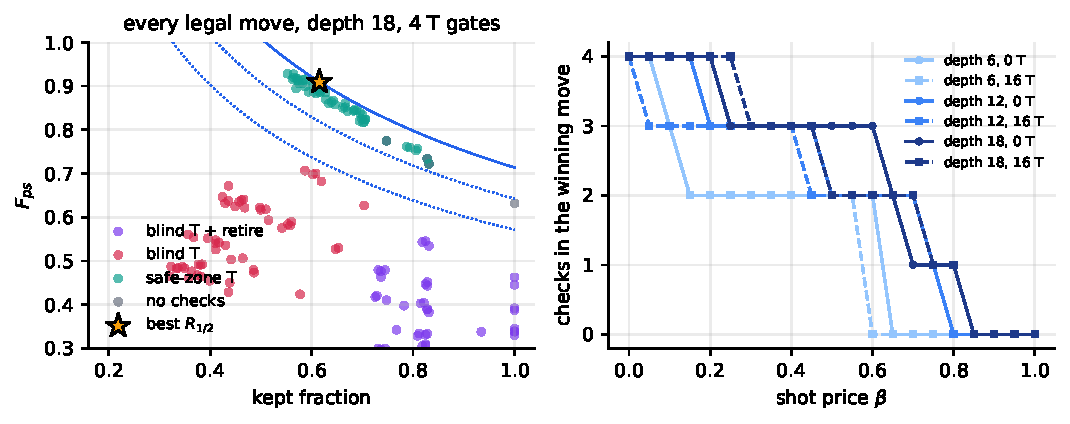
\includegraphics[width=0.9\textwidth]{figures/fig_pareto_beta}
\caption{Left: every legal move of the game's deep level with four $T$ gates. Lines are curves of constant $R_{1/2}$ through the best move (star) and at 90\% and 80\% of it. Right: number of checks in the winning move against the shot price $\beta$, for Clifford payloads (solid) and 16 $T$ gates (dashed).}
\label{fig:pareto}
\end{figure*}

\begin{figure}[t]
\centering
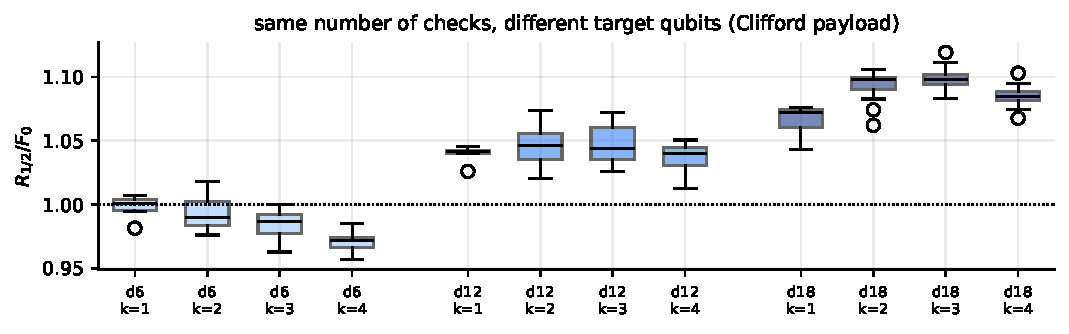
\includegraphics[width=\columnwidth]{figures/fig_location}
\caption{Check location. Fidelity-rate gain of every target set with $k$ checks on the Clifford payloads of the game.}
\label{fig:location}
\end{figure}

\subsection{Noise strength, noise model and noisy $T$ gates}
\label{sec:res-noise}
Figure~\ref{fig:noise} sweeps the two-qubit and readout error together from $10^{-3}$ to $3\times10^{-2}$, re-picking the checks at every point. With four checks at depth 18 the gain grows from \EfiveGainDeepLow{} at $p_2=10^{-3}$ to \EfiveGainDeepHigh{} at $p_2=3\times10^{-2}$. At depth 6 it stays below one at every noise level and even falls, from \EfiveGainShallowLow{} to \EfiveGainShallowHigh, because the checks' own gates get noisier along with everything else. Detection is most useful exactly when the circuit is too noisy to run well without it, and only when the circuit is deep enough for the payload to dominate the noise budget.

With the noise model derived from FakeFez calibration data, whose two-qubit error is about half that of the synthetic model, the same picture holds at smaller scale (Fig.~\ref{fig:profiles}): the best gain is \FezGainDeep{} at depth 18 with $k=\FezKDeep$ and \FezGainShallow{} at depth 6. Finally, if $T$ gates were not virtual but carried a depolarizing error of 1\%, the $T$ count would also lower the raw fidelity, from \EsevenFzeroHighTZero{} to \EsevenFzeroHighTSixteen{} at depth 12 (Fig.~\ref{fig:tnoise}). A $T$ gate sits on a Z-safe site, where every check flow acts as $I$ or $Z$, so the $Z$ part of its error is invisible to all checks and, wherever no flow passes, so is the rest. The post-selected fidelity therefore falls as well, from \EsevenFpsHighTZero{} to \EsevenFpsHighTSixteen. Safe sites are safe for the checks, not for the $T$ gates.

\begin{figure}[t]
\centering
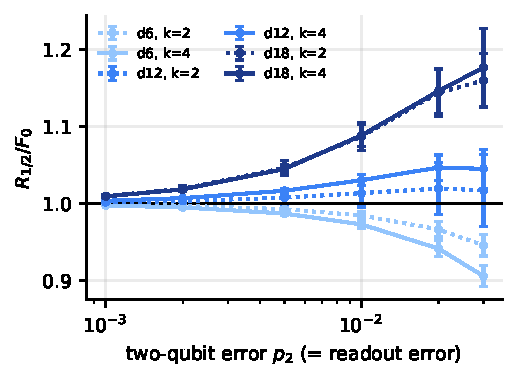
\includegraphics[width=\columnwidth]{figures/fig_noise}
\caption{Fidelity-rate gain against the two-qubit (and readout) error rate, for two and four checks at three depths. Checks are re-picked at every noise level.}
\label{fig:noise}
\end{figure}

\begin{figure}[t]
\centering
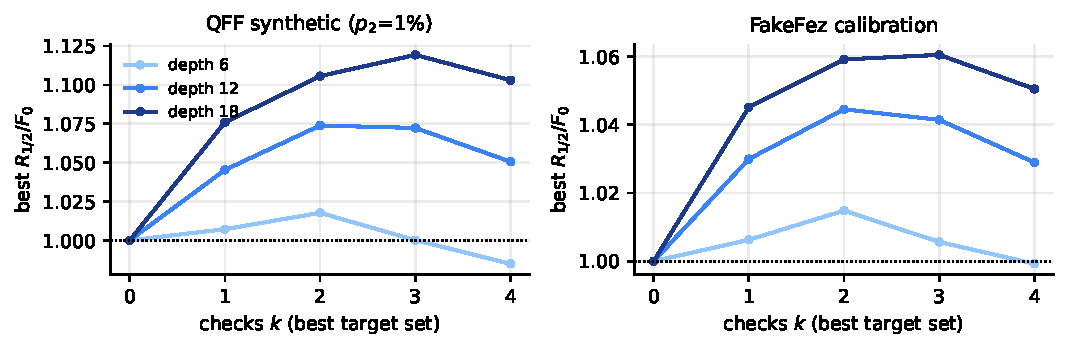
\includegraphics[width=\columnwidth]{figures/fig_profiles}
\caption{Best gain per number of checks for the two noise models (Clifford payloads of the game).}
\label{fig:profiles}
\end{figure}

\begin{figure}[t]
\centering
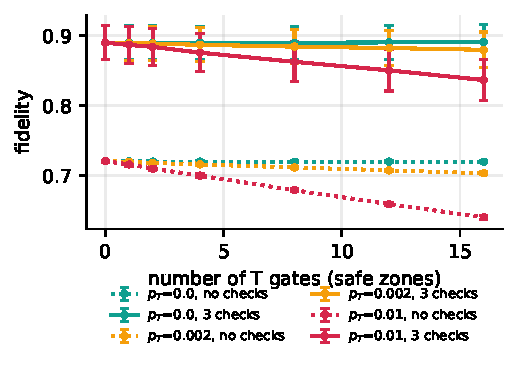
\includegraphics[width=0.8\columnwidth]{figures/fig_t_noise}
\caption{Ablation with noisy $T$ gates (depth 12, safe-zone doping). Dotted: no checks; solid: three checks.}
\label{fig:tnoise}
\end{figure}
